\documentclass[twoside, 12pt, a4paper]{refart}
\usepackage[utf8]{inputenc}
\usepackage[english]{babel}
%\usepackage[T2A]{fontenc} % это пакет с поддержкой русского
\usepackage{amsmath, amsfonts, amssymb, graphicx}
%\usepackage{pscyr} % это чтобы красиво было со шрифтами при подключении T2A
\usepackage{makeidx}
\usepackage{ifthen}
\usepackage{float}
\usepackage{hyperref}
\hypersetup{colorlinks=true,linkcolor=blue,filecolor=magenta,urlcolor=blue}
\urlstyle{same}

\renewcommand{\labelenumii}{\arabic{enumi}.\arabic{enumii}.}

\RequirePackage{caption}
\DeclareCaptionLabelSeparator{defffis}{ -- }
\captionsetup{justification=centering,labelsep=defffis}

\def\bs{\char'134 } % backslash in \tt font.
\newcommand{\ie}{i.\,e.,}
\newcommand{\eg}{e.\,g..}
\DeclareRobustCommand\cs[1]{\texttt{\char`\\#1}}

\title{Microfluidic pressure controller}
\author{
  Authors of the manual: \\
  Ivan A. Denisov \\
  Nikita A. Filatov \\
  Anton S. Bukatin \\
  % Лукьяненко Кирилл Андреевич \\
  % Сорокин Владимир Викторович \\
  % Якимов Антон Сергеевич \\
}



\date{9 Jan 2022}
\emergencystretch1em  %

\pagestyle{myfootings}
\markboth{Manual: Microfluidic pressure controller}%
         {Manual: Microfluidic pressure controller}

\makeindex 

\setcounter{tocdepth}{2}

\begin{document}

  \maketitle

  \begin{abstract}
    The manual includes instructions to assemble, setup and develop open-source microfluidic pressure controller. Additionally, the main stages of assembly of the device are indicated.
  \end{abstract}

  \tableofcontents

  \newpage


%%%%%%%%%%%%%%%%%%%%%%%%%%%%%%%%%%%%%%%%%%%%%%%%%%%%%%%%%%%%%%%%%%%%

  \section{Introduction}
    \label{intro}
    

    Controller has functions:
    \begin{enumerate}
      \item manual and program control 4 pressure outputs   
      \item manual and program control 1 vacuum pump
      \item control 8 relays for manage output devices
      \item control 4 digital inputs and 4 ADC (analog-to-digital converters)
      \item write automatic work protocols
    \end{enumerate}
 
    

    \begin{figure}[h!b]
	  \begin{center}
	  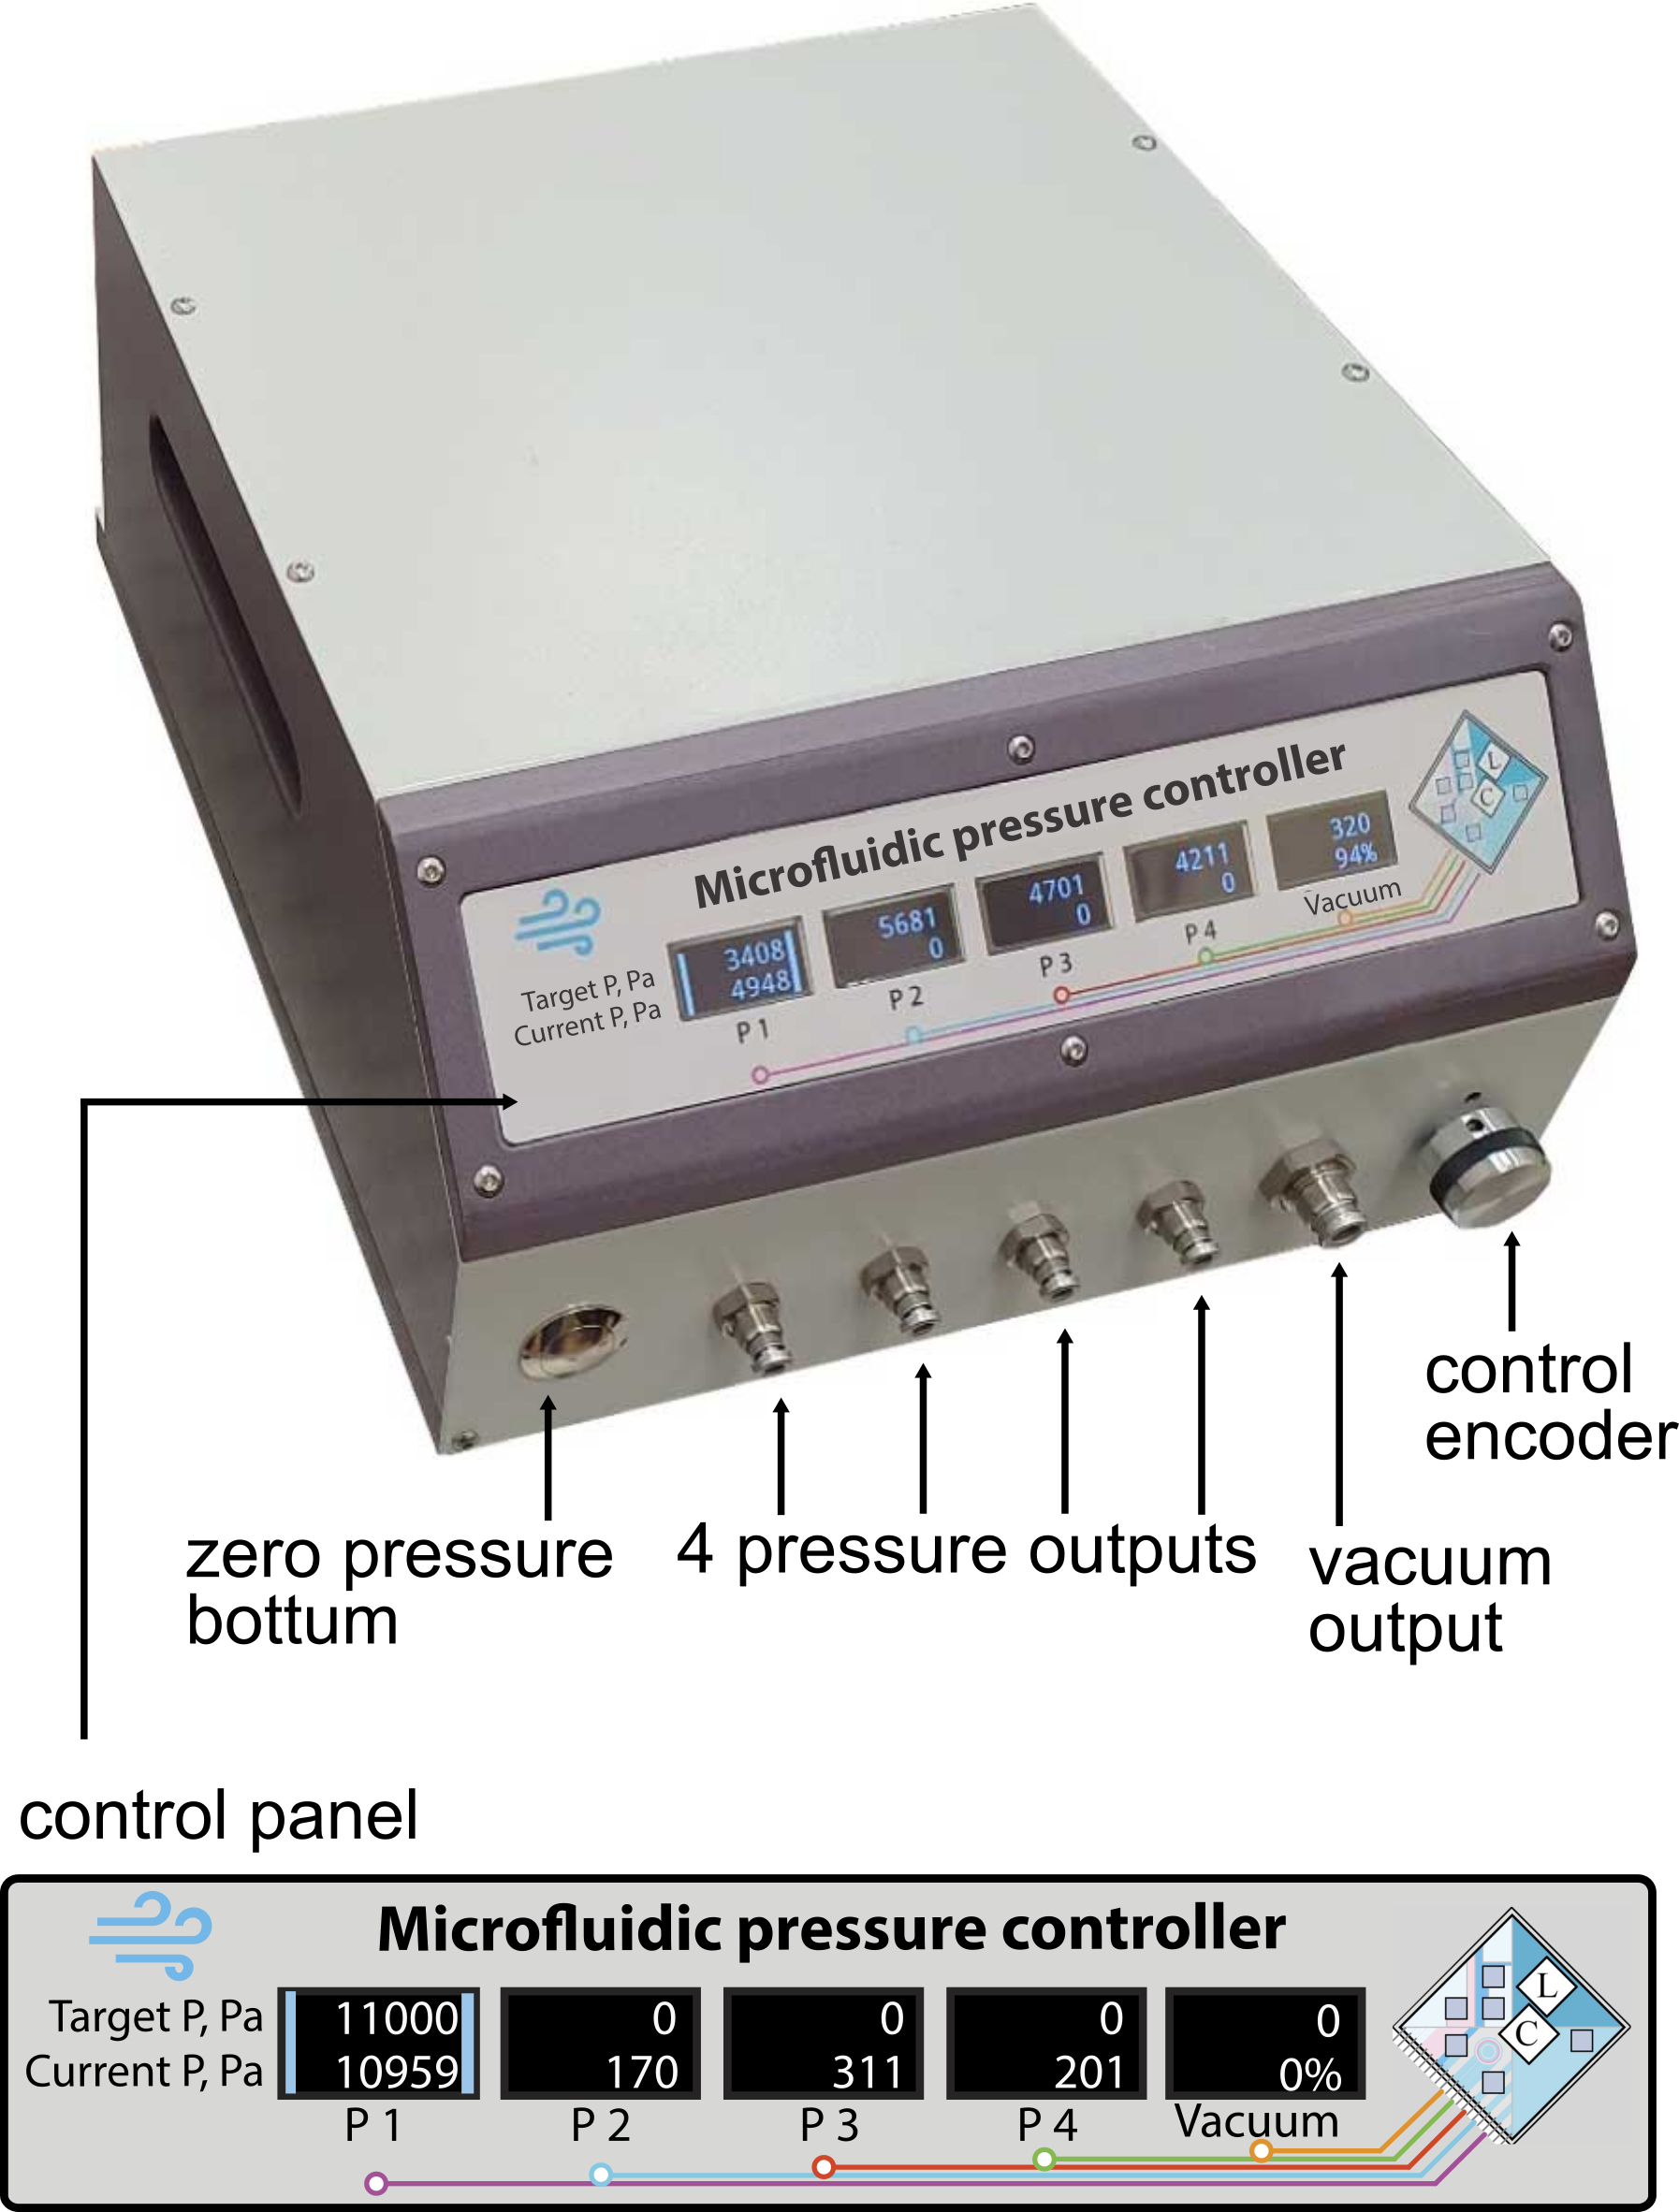
\includegraphics[width=\textwidth]{imgs/device.png}
	  \caption{General view of the microfluidic controller with 5 displays, 4 positive pressure outputs and 1 vacuum pump output}
	  \label{fig:device}
	  \end{center}
    \end{figure}


  \subsection{Transportation}
    The vacuum pump is attached to the body with silicone damping elements. So, to avoid damage to them, the device must be transported in a normal (horizontally) position, not turned on its side or upside down. For transportation in luggage it is necessary to fix the vacuum pump by removing the top cover of the device \footnote {for this you need to use a special hex bit, using an unsuitable tool may damage the screws and it will be impossible to unscrew them}
    
  \subsection{Storage}
    The device must be stored under conditions that do not lead to metal corrosion. Place plugs in all pneumatic ports: 1 pressure inlet and 5 pressure outlets. The absence of plugs will lead to the accumulation of microparticles, which can get into the microfluidic chip after the device is started up and lead to its malfunction. There is a filter inside the housing at the air inlet of the instrument, however we recommend that you follow the above precautions and install a plug on the inlet during long-term storage of the instrument.
    
%%%%%%%%%%%%%%%%%%%%%%%%%%%%%%%%%%%%%%%%%%%%%%%%%%%%%%%%%%%%%%%%%%%%%%
  \newpage
  \section{Setting up}
  \label{setup}
  
  \subsection{PC Software installation}
    \href{https://github.com/microfluidic-pressure-controller/software/releases}{Link to download the software application.}
    \newline If this link does not open:\\
    \url {https://github.com/microfluidic-pressure-controller/software/releases}
    
  \subsection{Software description}
    A USB 2.0 A / USB 2.0 B cable is required to connect the pressure controller to a computer.
    \newline General view of the menu panels is shown in the figure \ref{fig:menu panels}.
The following are the functions of the buttons and other elements:
      
    \begin{figure}[H]
	  \begin{center}
	  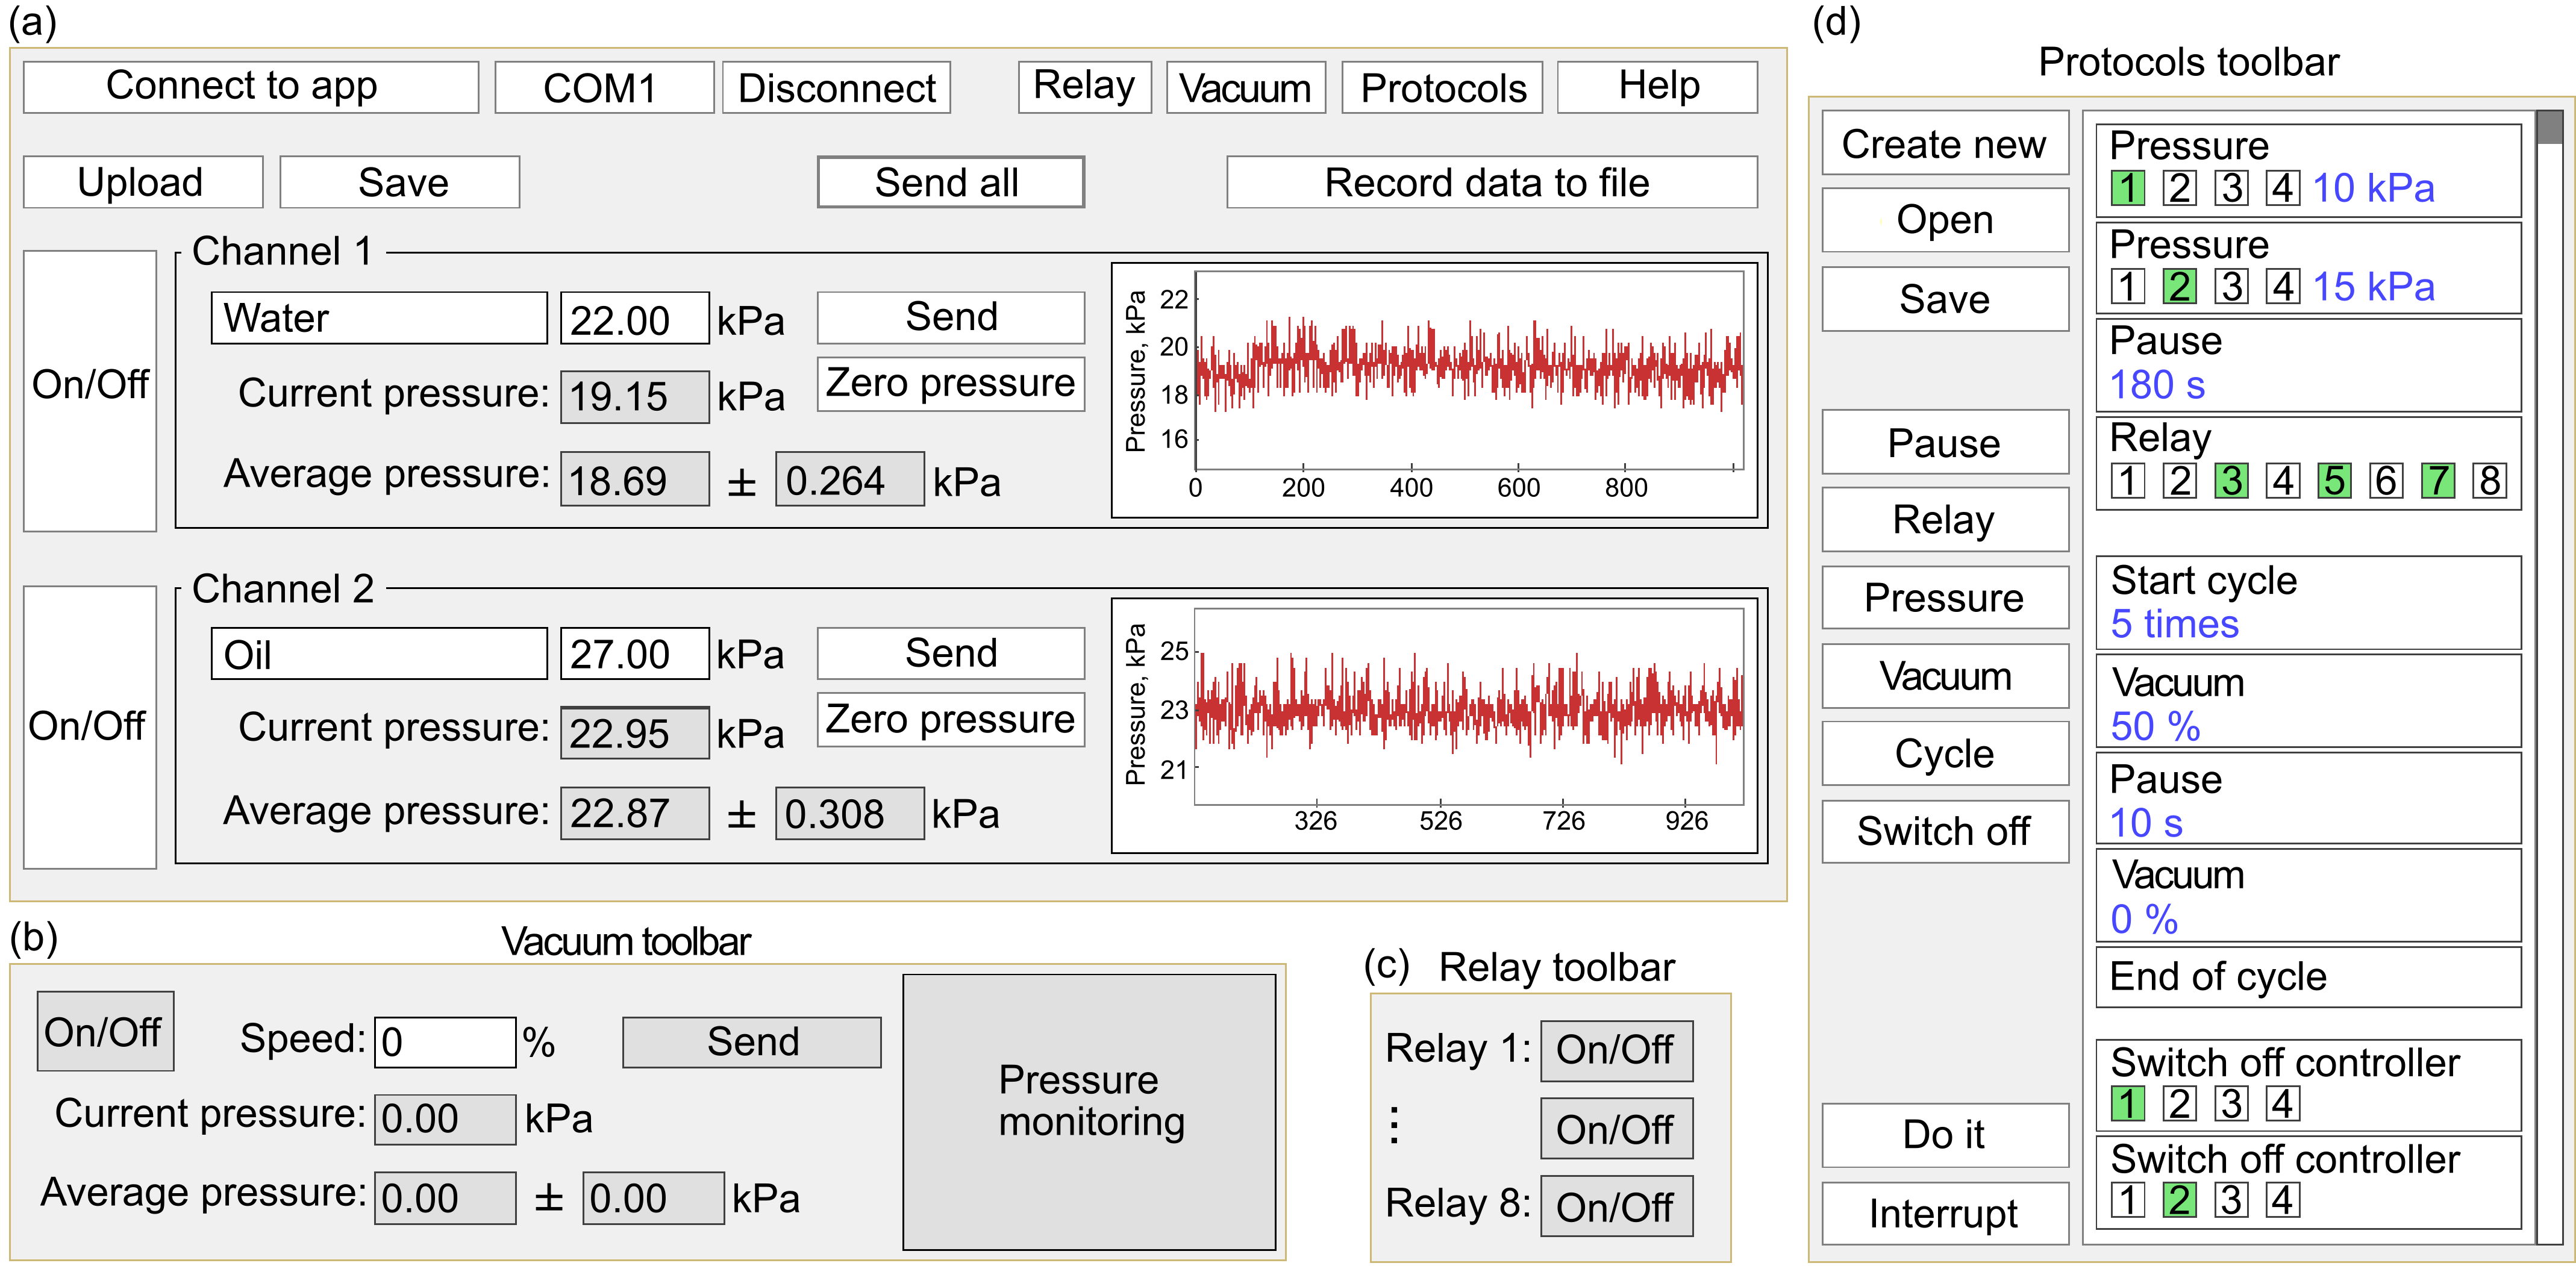
\includegraphics[width=\textwidth]{imgs/menu panels.png}
	  \caption{The software interface of the microfluidics pressure controller. (a) Main window of the interface that allows to control and monitor pressures in each channel. (b) Toolbar for controlling the integrated vacuum pump. (c) Toolbar for controlling external devices via relay outputs. (d) Toolbar for writing sequences for experiment automation.}
	  \label{fig:menu panels}
	  \end{center}
    \end{figure}
   
   
    \begin{description}
    \item[\textbf{Main menu}] figure \ref{fig:menu panels} a
    
      \marginlabel{Connect to app:} Pressing the "Connect to app" button establishes a connection to the pressure controller. Please note that disconnect occurs when you press the "Disconnect/or Close" button.
\newline Please note that when the application is launched, some of the buttons have a dark shade and cannot be pressed. This is a visual effect that the program has not established communication with the controller.
\newline If the COM port is selected correctly, then after pressing the "Connect to app", such dark buttons will become light and you can start controlling the controller.
\newline If the COM port is incorrect, the connection will not be made and the dark buttons will not become active. However, it may happen that if the port is incorrect, and when you click on "Connect to app", the dark buttons will turn light - and you will not be able to control the controller - you need to click "Disconnect/or Close", enter the correct port and click on "Connect to app" again (you may need to restart the program)
\newline If the COM port is selected correctly, but you cannot manage the controller, most likely you need to check the com port and restart the program.
      
      \marginlabel{COM i:} Enter the correct COM port to which the pressure controller is connected with a USB cable.
      
      \marginlabel{Disconnect (or Close):} Pressing the button terminates communication with the controller.
      
      \marginlabel{Relay:} Button to open the relay toolbar.
      
      \marginlabel{Vacuum:} Button to open the vacuum toolbar.
      
      \marginlabel{Protocols:} Button to open the Protocols toolbar.
      
      \marginlabel{Help:} Help, Tips, Calibration, Debugging, Contacts.  
          
      \marginlabel{Upload (or Load):} Button for loading saved program settings from the save-file.  
      
      \marginlabel{Save:} Button for saving all parameters of the program menu to a file: COM port number, signatures, pressures. The file will be saved in a folder with the Veterok.exe program.
      
      \marginlabel{Send all:} Command for sending pressure values to all channels at once. Hot key - press "Enter".
      
      \marginlabel{Record data to the file:} Command for writing data from sensors to a file: pressure on all 4 channels, negative pressure from the vacuum pump, conditional time. The conditional time must be recalculated in real time, taking as a basis the time when the recording to the file began and the time when the recording was stopped. Recording stops when you press the button again, but a new recording starts immediately. Also, the recording stops if you close the program or if you press "Disconnect/or Close".\\
      The name of the recording file displays the date (year-month-day) and real time (hour:minute:second) of its creation. For example: data\_2020-06-29\_13-48-30.csv.
      
      \marginlabel{On/Off:} Enable / Disable ITV Pressure Controllers.
      
      \marginlabel{Channel 1,2,3,4:} Signatures to pressure channels. Below a caption there is a white field for entering the name of a channel, for example, "disp.phase - water\_1". 
      
      \marginlabel{Send} Command to supply the set new pressure value.  
            
      \marginlabel{Zero pressure} Command to supply zero pressure value (0 kPa). 
                  
      \marginlabel{Graphic pressure sensor data} It is a window where for each individual ITV controller channel a graph of pressures from a pressure sensor is displayed depending on a conditional time. \\ 
               
            
    \item[\textbf{Vacuum toolbar}] figure \ref{fig:menu panels} b
      
      \marginlabel{On/Off} Enable / Disable vacuum pump. 
      
      \marginlabel{Speed} Text field for setting a pumping force in percent 0-100\%.  
            
      \marginlabel{Send} Command to supply the set new speed value.     
    
    \item[\textbf{Relay toolbar}] figure \ref{fig:menu panels} c
    
      \marginlabel{On/Off} Enable / Disable relay. A total of 8 relays can be controlled.  
        
    \item[\textbf{Protocols toolbar}] figure \ref{fig:menu panels} d
      
      In the protocols menu, you can create an algorithm for the automatic operation of the microfluidic pressure controller yourself. Figure \ref{fig:menu panels} d shows a sample code.
      
      \marginlabel{Create new} Command to create a new protocol.
      
      \marginlabel{Open} Command to open saved protocol.  
      
      \marginlabel{Save} Command to save protocol.  
      
      \marginlabel{Pause} Pause operator. 
       
      \marginlabel{Relay} Relay operator. 
       
      \marginlabel{Pressure} Pressure operator. You can select a channel or channels and set them a pressure value.  
      
      \marginlabel{Vacuum} Negative pressure operator. You can set speed value of the vacuum pump.  
      
      \marginlabel{Cycle} Cycle operator. You can set the number of execution cycles. Required commands are placed inside the loop.  
      
      \marginlabel{Switch off} Command to power off one of pressure channels.  
      
      \marginlabel{Do it} Command to run the protocol. 
      
      \marginlabel{Interrupt} Command to stop the protocol.  

     
    \end{description}     
  
  \subsection{Calibration pressure sensors and adjustment ITV pressure rage}
    
    \textbf{Attention!} Further information for developers. Use it competently. Incorrect use can confuse instrument settings.\\
    Calibration and adjustment ITV pressure rage of the instrument is performed in the Help menu of the application.\\
    
    Please note that different ITV models (therefore different pressure ranges) can be built into a microfluidic pressure controller. For example, ITV0010 has 0.001 - 0.1 MPa output pressure range. ITV0030 has 0.001 - 0.5 MPa. Therefore, it must be observed that the range in the application (microcontroller firmware) matches the range of the installed ITV regulators.\\
    
    Note that the instrument has a special DAC (digital to analogue converter) connection through a current limiting resistor, so the maximum value of a pressure range is never reached. Therefore, the ITV range must first be determined with an external measuring device.\\
    
    Note that DAC is powered by 5V, and operates in 5 volt range. In this case, the entire ITV pressure range can be used. But if you use the working range of DAC as 3.3V, then the accuracy of pressure regulation increases up to 2 times, but the pressure range is reduced and becomes about 66\% of the total \footnote{compare 12bit/5V with 12bit/3.3V}. For example, for 100 kPa, only up to 66 kPa can be used.
        
    \marginlabel{Adjustment ITV pressure rage:}
      \begin{enumerate}
        \item Open the application \textbf{Veterok.exe}, press bottom "Help" and find the button "Calibration".    
        \item Set the maximum pressure value on the channel, which is allowed by the control panel of the controller and press the "Send" button. This will supply the maximum voltage value (maxP). Knowing this value of maxP in Pascals, calculate the coefficient using the formula maxP [Pa] / 4095 * 100.
        \item This coefficient must be specified for the corresponding channel through the calibration control panel: press the "Calibration" button or go to this "Calibration" window.
        \item Enter the coefficient in the appropriate field.
        \item Repeat instructions for other ITV regulators.
      \end{enumerate}
     
      
         
    \marginlabel{Calibration pressure sensors:}
      \begin{enumerate}    
        \item Open the application \textbf{Veterok.exe}
        \item Press bottom "Help" 
        \item Find and press the button "Calibration".  
        \item Choose one of the pressure regulators.
        \item Connect the selected pressure output to the pneumatic input of the measuring device (water column, pressure gauge, vacuum gauge or other sensor).\\
ATTENTION! When calibrating using the height of the water column, be careful not to allow water to enter the pressure controller. Use an intermediate container of sufficient volume, where water will leak in case of an error, but not too large, so that the compressed air does not have a significant effect on the measured values. In the "Calibration" menu, there is a handy calculator for working with the water column.
        \item Open if closed the calibration control panel - press the button "Calibration" in "Help" menu.
        \item In the "Calibration" control panel there is "Configuring pressure sensors", using the "Request coefficients" button, request the current coefficients that are saved in the device.\\
The coefficients sensA, sensB have the following meaning: p [Pa] = ADC x sensA + sensB\\
ADC can be an integer from 0 to 4095 - this is data from pressure sensors.
The sensA and sensB coefficients are used to calculate the pressure in Pascals from the 12-bit ADC values.\\
Please note that for each analog pressure sensor in the documentation, some voltage conversion factors are indicated, which most often can be reduced to the form: y = kx + b however, given that the device can use voltage dividers, it is not always possible to calculate specific factors sensA and sensB without experimental measurements.
        \item If you are calibrating a new sensor:
          \begin{enumerate} 
            \item Set sensA = 1 [Pa/bit] and sensB = 0 [Pa], then the monitors will display just p = ADC, where ADC = integer number from 0 to 4095. Take at least three different measurements (different pressure values) from the external sensor p [Pa] depending on ADC [0-4095]. Plot this graph and approximate it with a linear dependence (it is convenient to use OriginPro 8 or a later version). This will find the dependence p [Pa] = kx + b, or p [Pa] = ADC x sensA + sensB. In this way, the coefficients corresponding to the real ones sensA and sensB will be found.
ATTENTION! To calibrate the coefficients more accurately, you can use measurements not by sensors, but by the readings of the water column in the capillary (note the warning above about water columns)
            \item Enter the found sensA and sensB in the menu "Setting pressure sensors" in the fields corresponding to the output of the pneumatic interface (from top to bottom = 1 - 4 controller outputs, the 5th is the output of the vacuum pump). And click the "Submit" button below the fields and formulas. The pressure controller will show all values based on the new coefficient values.
            \item If you want to clarify the sensA and sensB coefficients, then you should use the method of selection of values below:
          \end{enumerate} 
        \item If the sensors have already been calibrated and you want to clarify the sensA and sensB coefficients, then you should use the method of selection of values below:
          \begin{enumerate} 
            \item Set the target pressure on the instrument control panel

            \item Calculate the difference between the pressure displayed on the panel and the actual pressure that you measured with an external meter.

            \item The resulting difference must be added to the sensB coefficient, and then send it to the controller using the "Send" button

            \item If the values start to coincide, then in this case save to the controller memory using the "Flash" button.

            \item Steps 1-3 must be repeated several times for different pressures to ensure linearity over the operating range.
            
          \end{enumerate}
      \end{enumerate}
        
   
%%%%%%%%%%%%%%%%%%%%%%%%%%%%%%%%%%%%%%%%%%%%%%%%%%%%%%%%%%%%%%%%%%%%%%

  \newpage
  \section{Usage manual} 
  \label{usage}

    Device can be controlled with physical panel on the front part of the device box with or without PC (personal computer) application.

  \begin{description}
    \item[\textbf{Control panel}] figure \ref{fig:device} 
    
    \marginlabel{Encoder:} Device has encoder to change settings. Simply twisting the encoder knob displaces the vertical band (a kind of indicator) from display to display.\\
If you leave a vertical band on the desired display and press the encoder, a second vertical band will appear on the left, which means that the display (device) is selected and values can be set.
The values are set by rotating the encoder.
To apply a value, you need to press the encoder and hold it for 3-5 seconds.
To exit the selected screen, you just need to press the encoder 1 time.
    
    \marginlabel{Displays:} Displays informing about target and current pressures. The current pressure is the pressure from the sensor. Also, a vertical band may appear on each display. If it is displayed on the right, it means that now the encoder pointer is on this display (device). If the vertical band is not displayed, then the encoder is pointing to another display (device). If vertical bands are displayed both on the left and on the right hands, then the display (device) is selected and you can operate it.
    
    \marginlabel{Zero pressure buttom:} Pressure reset button to zero 0 kPa.
    
  \end{description}

%%%%%%%%%%%%%%%%%%%%%%%%%%%%%%%%%%%%%%%%%%%%%%%%%%%%%%%%%%%%%%%%%%%%%%
  \newpage
  \section{Developing application}
    If you wish, you can assemble such a pressure controller yourself.\\
    All the designs, circuit diagrams, and software are published on  \href{https://github.com/microfluidic-pressure-controller}{GitHub} (https://github.com/microfluidic-pressure-controller).\\
  
    In brief, the following is a description of the main subassemblies.
    
    The figure \ref{fig:mainscheme} shows a general diagram of the functioning of a microfluidic pressure controller.
    
    \begin{figure}[H]
	  \begin{center}
	  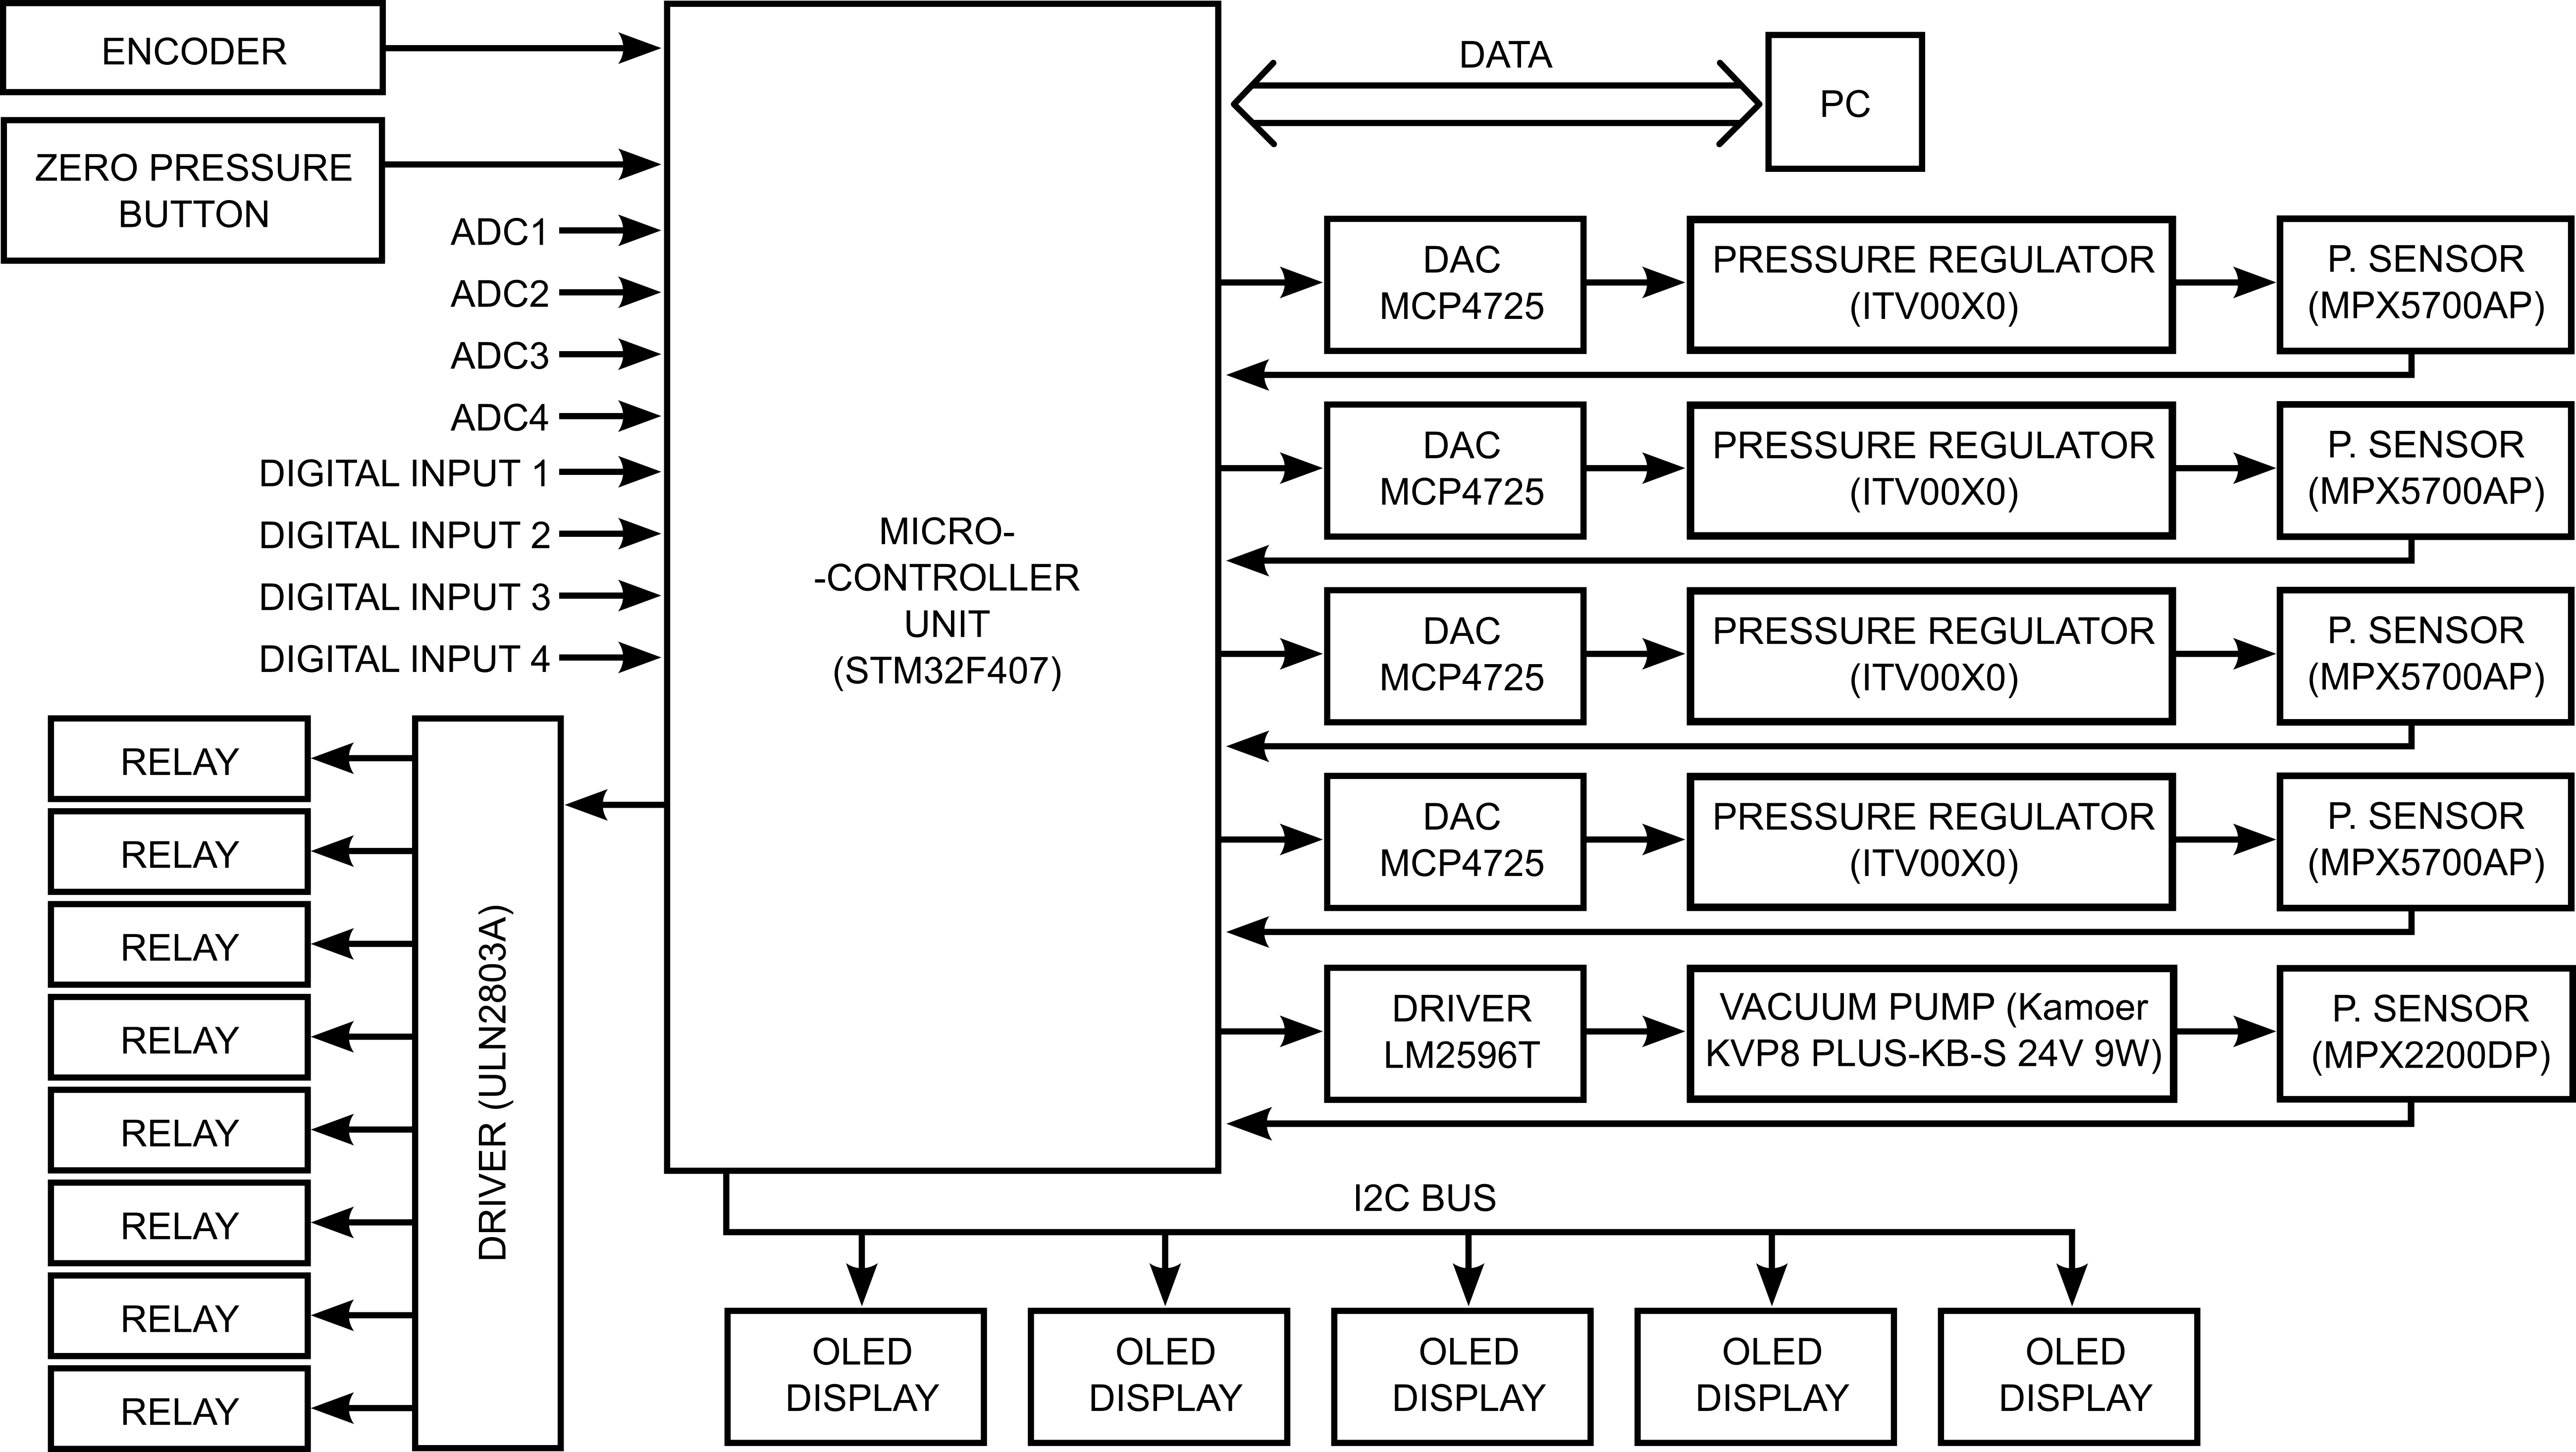
\includegraphics[width=\textwidth]{imgs/main-scheme.png}
	  \caption{The electric circuit diagram of the pressure controller.}
	  \label{fig:mainscheme}
	  \end{center}
    \end{figure}
    
    An internal overview of the components of the microfluidic pressure controller is shown in figure \ref{fig:device-structure}, \ref{fig:device-structure2}.
    \begin{figure}[H]
	  \begin{center}
	  \includegraphics[width=\textwidth]{imgs/device-structure.png}
	  \caption{An internal overview of the components of the microfluidic pressure controller: (a) side view; (b) back view.}
	  \label{fig:device-structure}
	  \end{center}
    \end{figure}
    
    \begin{figure}[H]
	  \begin{center}
	  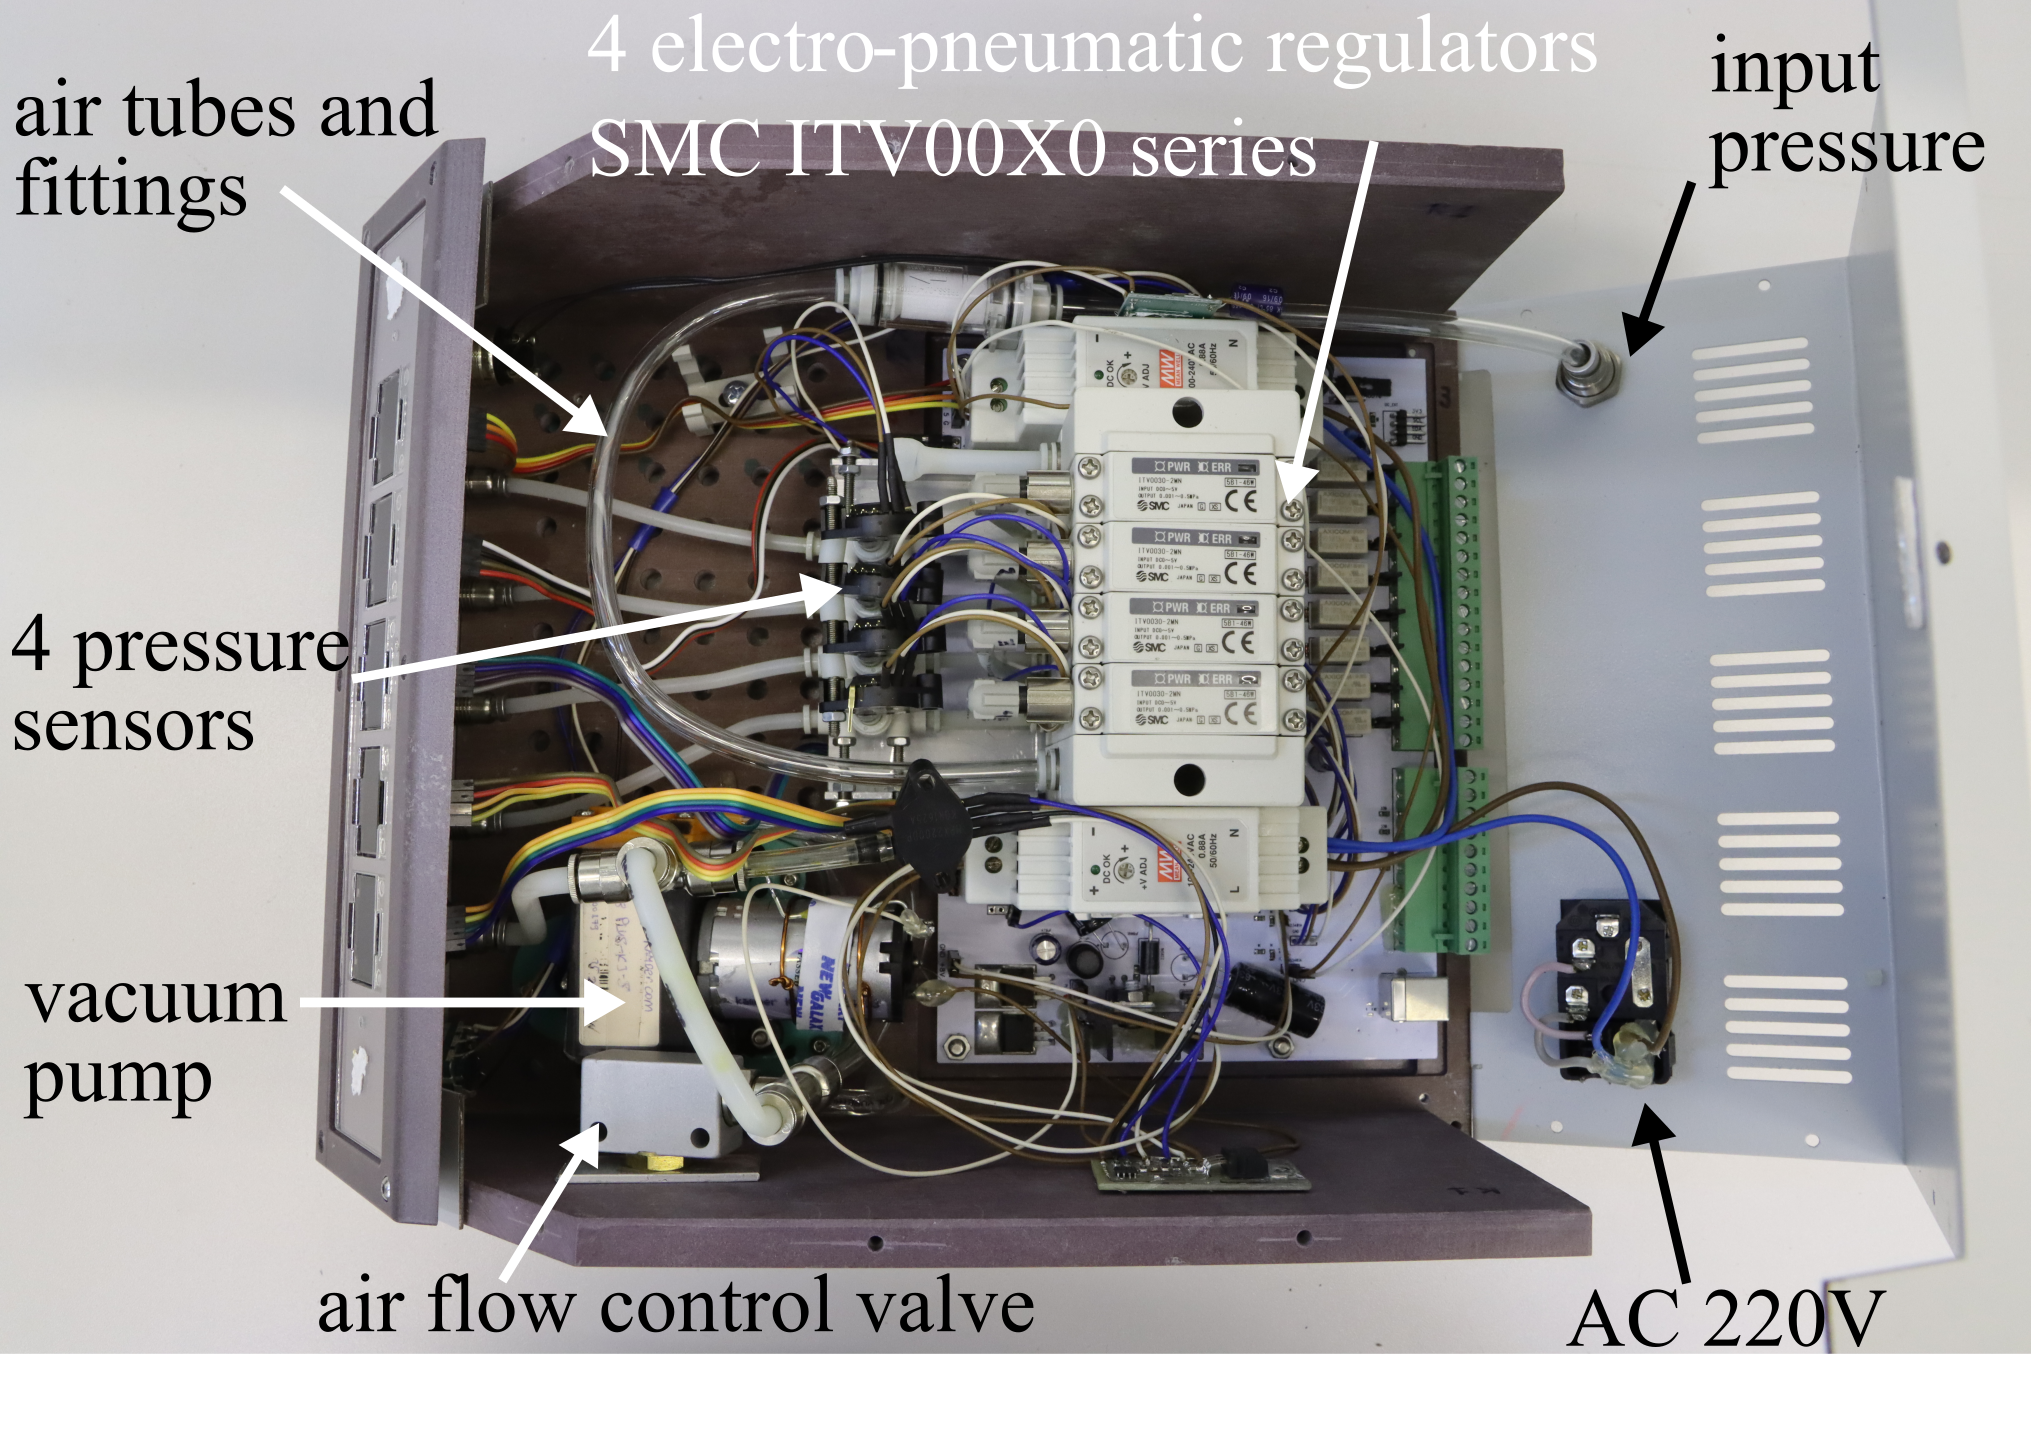
\includegraphics[width=\textwidth]{imgs/device-structure2.png}
	  \caption{An internal overview of the components of the microfluidic pressure controller: top view.}
	  \label{fig:device-structure2}
	  \end{center}
    \end{figure}
  
  
  
  
  
  
  
  
  
  
  
  
  
  
  
  
  
  
%%%%%%%%%%%%%%%%%%%%%%%%%%%%%%%%%%%%%%%%%%%%%%%%%%%%%%%%%%%%%%%%%%%%%%
  \newpage
  \section{ATTENTIONS}
    \begin{description}  
    \item[Vacuum pump]
      If you set such a power that will stop the pump, it may overheat and fail. The device is equipped with protection against fire (a thermal fuse is attached to the pump motor), however, system operation is irreversible without repairing the device (replacing the thermal fuse).
    \end{description} 




\printindex

\end{document}
